% Plantilla común para figuras redibujadas (fig-NN-desc.tex).
% Copiar entera y sustituir solo el cuerpo entre las marcas "cuerpo de la figura".
% Compila tal cual en Overleaf o con scripts/tikz2svg.sh.
%
% NO añadir la opción "tikz" a standalone: parte cada tikzpicture (y cada
% \chemfig) en una página distinta y el SVG solo tendría la primera.
\documentclass[border=4pt]{standalone}
\usepackage[T1]{fontenc}
\usepackage{lmodern}            % base vectorial: sin fuente vectorial el texto sale en Type 3 y dvisvgm lo pierde
\usepackage[scaled=0.95]{helvet}% sans-serif tipo Helvetica, como la interfaz de Obsidian
\renewcommand{\familydefault}{\sfdefault}
\usepackage{amsmath,amssymb}
\usepackage{sansmath}\sansmath  % fórmulas en sans, a juego con el texto
\usepackage[version=4]{mhchem}  % \ce{A + B -> C}
\usepackage{chemfig}            % estructuras y esquemas de reacción
\usepackage{graphicx}           % \includegraphics de recortes vectoriales (rec-NN.pdf)
\usepackage{tikz}
\usetikzlibrary{arrows.meta,positioning,calc,shapes.geometric,decorations.pathmorphing,decorations.markings}
\usepackage{pgfplots}           % gráficas (cinética, curvas de valoración...)
\pgfplotsset{compat=1.18}

% ---- Estilo Apuntes.md --------------------------------------------------
% Paleta semántica (la misma que el CSS de Obsidian). Principios inspirados en
% figures4papers (ChenLiu-1996, CC BY-NC 4.0): se adoptan ideas, no código.
\definecolor{apAzul}{HTML}{0F4D92}       % anotaciones, estructura (el azul del autor)
\definecolor{apAzulClaro}{HTML}{3775BA}
\definecolor{apRojo}{HTML}{B64342}       % curvas y datos principales, importante (el rojo del autor)
\definecolor{apRojoClaro}{HTML}{E9A6A1}
\definecolor{apVerde}{HTML}{3B7D3B}      % definiciones, "positivo"
\definecolor{apVerdeClaro}{HTML}{AADCA9}
\definecolor{apGris}{HTML}{767676}       % apoyo: rejillas, referencias, líneas punteadas
\definecolor{apGrisClaro}{HTML}{CFCECE}
\definecolor{apNegro}{HTML}{272727}      % ejes y texto neutro

\tikzset{
  % sin "color=" global: pisaría los \color{...} de chemfig (estructuras en rojo, etc.)
  every picture/.append style={line width=0.9pt, >={Stealth[length=2.4mm]}},
  curva/.style={apRojo, line width=1.6pt},                  % la curva o el dato que importa
  curva secundaria/.style={apAzulClaro, line width=1.3pt},
  referencia/.style={apGris, dotted, line width=1pt},       % líneas guía (p. ej. y = 0)
  anotacion/.style={apAzul, font=\normalsize},              % texto escrito a mano alrededor del dibujo
  flecha/.style={->, apAzul, line width=1pt},
  implica/.style={-{Implies}, double, double distance=2pt, line width=0.8pt},
  marca/.style={circle, fill=apAzul, draw=white, line width=0.6pt, inner sep=1.8pt},
  resalte/.style={apAzul, line width=1pt},                  % círculos/óvalos que rodean algo
}
\pgfplotsset{
  apuntes/.style={
    axis lines=left, axis line style={line width=1pt, apNegro, -{Stealth[length=2.4mm]}},
    tick style={apNegro, line width=0.8pt}, tick align=outside,
    label style={font=\normalsize}, tick label style={font=\normalsize},
    every axis plot/.append style={curva},
    clip=false,
  },
}
\setchemfig{atom sep=2em, bond style={line width=0.9pt}}
% -------------------------------------------------------------------------

\begin{document}
% --- cuerpo de la figura ---
% Los 4 niveles de estructura de las proteínas (pág. 8)
% iconos: Protein_primary/secondary/tertiary/quaternary_structure (DBCLS, CC-BY 4.0)
\begin{tikzpicture}[font=\normalsize]
  % ---- Primaria: los 4 primeros residuos del icono, en vertical, con sus nombres
  \node[inner sep=0] (p) at (0,0.35) {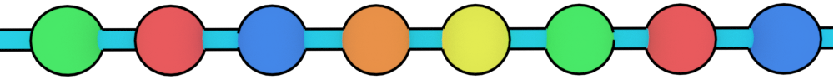
\includegraphics[trim=0 0 200 0, clip, angle=-90, totalheight=3.2cm]{ico-01-primaria.pdf}};
  \begin{scope}[x={($(p.south east)-(p.south west)$)}, y={($(p.north west)-(p.south west)$)}, shift={(p.south west)}]
    \foreach \r/\v in {Pro/0.86, Ala/0.61, Asp/0.36, Cys/0.11} {
      \node[anchor=west, apVerde] at (1.3,\v) {\r};
    }
  \end{scope}
  \node[anotacion, align=center] at (0,2.6) {Secuencia de\\residuos};
  \node[apRojo] at (0,-1.75) {Primaria};
  % ---- Secundaria
  \node[inner sep=0] (s) at (4.0,0.35) {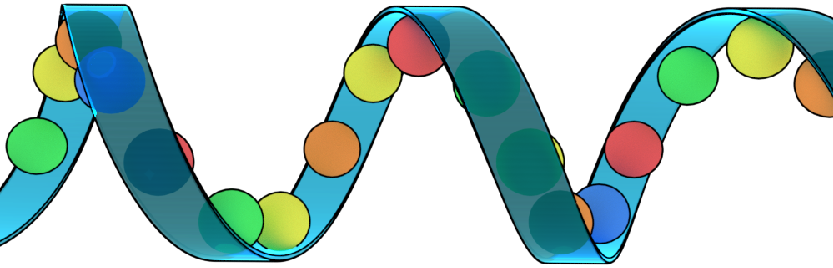
\includegraphics[width=3.4cm]{ico-02-secundaria.pdf}};
  \node[anotacion, align=center] at (4.0,2.6) {Estructura local de\\la cadena principal};
  \node[apRojo] at (4.0,-1.75) {Secundaria};
  % ---- Terciaria, con la hélice rodeada en rojo como en la hoja
  \node[inner sep=0] (t) at (8.2,0.35) {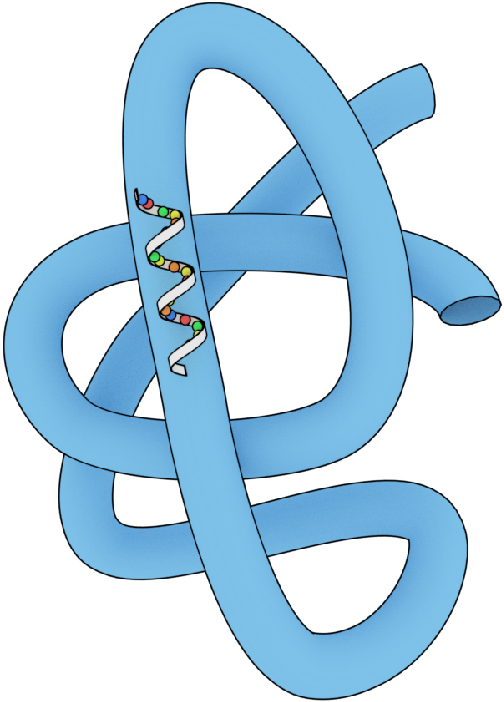
\includegraphics[height=3.2cm]{ico-03-terciaria.pdf}};
  \begin{scope}[x={($(t.south east)-(t.south west)$)}, y={($(t.north west)-(t.south west)$)}, shift={(t.south west)}]
    \draw[resalte, apRojo, line width=1.4pt] (0.33,0.58) ellipse (0.2 and 0.17);
  \end{scope}
  \node[anotacion, align=center] at (8.2,2.75) {Estructura global de\\una sola cadena\\polipeptídica};
  \node[apRojo] at (8.2,-1.75) {Terciaria};
  % ---- Cuaternaria, con una cadena rodeada en rojo como en la hoja
  \node[inner sep=0] (c) at (12.4,0.35) {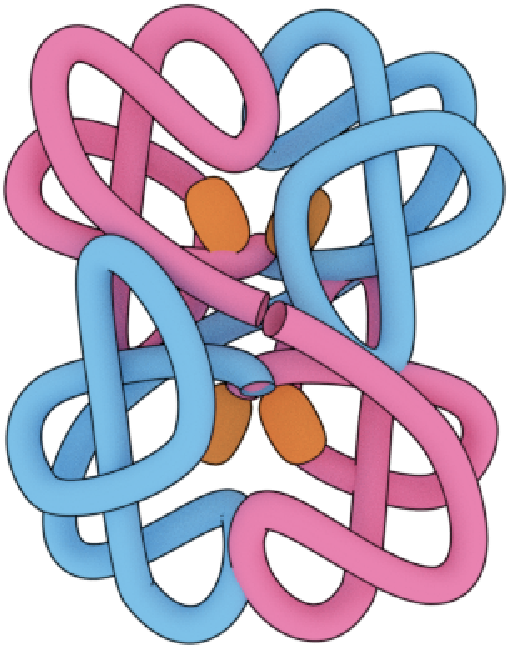
\includegraphics[height=3.2cm]{ico-04-cuaternaria.pdf}};
  \begin{scope}[x={($(c.south east)-(c.south west)$)}, y={($(c.north west)-(c.south west)$)}, shift={(c.south west)}]
    \draw[resalte, apRojo, line width=1.4pt] (0.31,0.73) ellipse (0.31 and 0.28);
  \end{scope}
  \node[anotacion, align=center] at (12.4,2.75) {Estructura global de un\\oligómero de\\varias cadenas};
  \node[apRojo] at (12.4,-1.75) {Cuaternaria};
  % ---- flechas entre niveles
  \draw[->, apRojo, line width=1.2pt] (1.3,0.35) -- (2.15,0.35);
  \draw[->, apRojo, line width=1.2pt] (5.85,0.35) -- (6.95,0.35);
  \draw[->, apRojo, line width=1.2pt] (9.45,0.35) -- (11.15,0.35);
\end{tikzpicture}
% ---------------------------
\end{document}
